\documentclass[conference]{IEEEtran}
\IEEEoverridecommandlockouts
% The preceding line is only needed to identify funding in the first footnote. If that is unneeded, please comment it out.
\usepackage{cite}
\usepackage{amsmath,amssymb,amsfonts}
\usepackage{algorithm}
\usepackage{algpseudocode}
\usepackage{graphicx}
\usepackage{textcomp}
\usepackage{xcolor}
\def\BibTeX{{\rm B\kern-.05em{\sc i\kern-.025em b}\kern-.08em
    T\kern-.1667em\lower.7ex\hbox{E}\kern-.125emX}}
\usepackage{graphicx}
\graphicspath{ {./images/} }

\begin{document}

\title{Medical Image Tamper Detection}
\author{
  \begin{tabular}{ c c c c } % number of c's = number of cols
    \shortstack{Zack Muraca\\
    Cal Poly, Pomona\\ CS 4210}
 &
   \shortstack{Gary Kim\\
    Cal Poly, Pomona\\ CS 4210} % also deleted newline chars here
&
    \shortstack{Thongsavik Sirivong\\
    Cal Poly, Pomona\\ CS 4210}
 &
   \shortstack{Nhat Tran\\
    Cal Poly, Pomona\\ CS 4210}
\end{tabular}
    }
\maketitle


\begin{abstract}
Today, a CT (Computed Tomography) scanner is an essential tool in health-care systems. CT scans are used to diagnose certain diseases (e.g., heart disease, trauma, infectious diseases, cancer, etc.) In 2020, health-care systems were attacked brutally leading to treatment interruptions and medical record breaches. Concerning the influential aspects of medical data, we will have to focus on inproving the security of health-care systems. In this research, we use a deep learning machine learning algorithm to detect tampered medical images.
\end{abstract}


\section{Introduction}
Medical technology has improved significantly in the recent decades. Technology like 3D medical imaging has allow healthcare professionals to access new angles, resolutions and details to diagnose certain medical conditions. There are few common techniques for producing detailed 3D medical imagery. One of the techniques is CT (Computed Tomography). CT scanners use X-Rays to take many 2D scans of the body over the axial plane along the body to create 3D images. The data from CT scans are managed through a picture archiving and communication system (PACS), which is an Ethernet-based network involving a central server that stores/retrieves the scans in/from a database, using the standardized DICOM format \cite{study}. As the medical technology expands, the health-care security policies tends to address data privacy more than data security. McAfee researchers found that some of the medical facility's web portals can be exploited to view and modify a patient's 3D DICOM imagery. Though, PACS is a local server system, it is indirectly connected to the facility's internal network. Also, they are vulnerable to social engineering attacks, physical access, and insiders \cite{study}. With medical imagery falling into the wrong hand, an attacker can alter the image, such as add or remove evidence of some medical condition, to cause a misdiagnosis. In this research, we will be looking into a dataset of tampered scans and come up with a predictive model, with deep learning algorithms, that is capable of determining whether the medical 3D scanned images are tampered images, or originally scanned images.

\section{Dataset}
Our data consists of two sets: the tampered scans and the original scans. The original scans being the ones used by \cite{study} which are the true images such that they have not been altered, indicating whether patients really have cancer or not, and the tampered scans are the images altered by the same authors which are not guaranteed to be altered but can be, indicating there exists false positives and false negatives. Each scan in our two datasets consists of hundreds of images, with an average around two hundred, and each image has a consistent resolution of 512 by 512 pixels. If a scan has been tampered with, any amount of these pixels will be altered per image, including zero. This will certainly prove to be a challenge throughout the duration of this project, along with mapping each scan in the original, untampered dataset with its corresponding tampered scan in the dataset used by \cite{study}.

\section{\textbf{Methodology}}
The goal is to learn $f : X \longrightarrow \hat{y}$ and $Loss(y, \hat{y})$ is low, where $X$ is the set of 3D lung CT scans with dimension $Depth \times Width \times Height$, and $\hat{y},\ y \in \{tampered, not\ tampered\}$ are predicted labels and ground truth labels. The loss function we used was binary cross entropy and an Adam optimizer was used. Training occurred over a maximum of 200 epochs with a patience of 30 epochs (i.e. if no improvements are made in 30 epochs, save the best model and terminate training.)
\subsection{\textbf{Uniform Data Transformation}}
The data consists of slices of dimensions $512 \times 512$. However, each instance consists of a varying number of slices in the range of $[80, 500]$. To transform the data to have equal dimensions, the following slice selection techniques were considered:

\textit{Subset Slice Selection (SSS)}: Slices are sampled from different regions of the the entire depth; generally, sampling happens at the beginning, middle, and end of the depth. The depth samples are then concatenated to form a new 3D scan that matches our desired dimensions.

\textit{Even Slice Selection (ESS)}: The biggest problem with SSS is that, since sampling only happens at a small number of slices, a lot of information is lost in the unsampled slices, which is discarded. ESS is a specific case of SSS where sampling is done at every $F$ slices, where $F$ is the space factor, $D$ is the depth, $N$ is the desired depth. $F = \frac{D}{N}$. By maintaining this space factor throughout the sampling, the resulting scan is more representative of the overall 3D scan than the one produced by SSS.

\textbf{\textit{Spline Interpolated Zoom (SIZ)}}: While ESS is an improvement over SSS, the technique used in the research is SIZ. SIZ better represents the original 3D scan than ESS because ESS ultimately samples from a subset of slices. In this technique, the given 3D scan is zoomed along the depth dimension by a factor of $\frac{N}{D}$ using spline interpolation. The end result is that the input scan is zoomed by replicating the nearest pixel along the depth dimension [3].

\begin{algorithm}
\caption{Spline Interpolated Zoom [3]}\label{alg:cap}
\begin{algorithmic}
\Require A 3D scan $I$ of dimensions $D \times W \times H$.
\Ensure $I$ is a rank 3 tensor.\\
1. Set constant desired depth of size $N$.\\
2. Determine depth by counting the number of slices.\\
3. Compute depth factor, $DF = \frac{1}{D/N}$.\\
4. Zoom $I$ using spline interpolation by factor $DF$.\\
5. Output transformed scan $I'$ of dimension $N \times W \times H$.\\
\end{algorithmic}
\end{algorithm}


\subsection{\textbf{Three-dimensional (3D) CNN architecture}}
\par
The first model trained had a regular deep learning architecture. This was very inefficient and impractical for the dataset which contains hundreds of slices per instance. This led to extremely long training times, which limited the training to just 10\% of the full dataset. Consequently, our initial model not only could not generalize to the test set, but was also underfitting the training set.
\par
Our final model uses the architecture used in a different research to predict tuberculosis from 3D CT scans. This choice was made for the following reasons: 
\begin{itemize}
    \item Since CNN's downsample the data across the hidden layers, the training time should be smaller than a regular deep learning model. 
    \item Both tasks deals with binary classification from medical 3D CT scans and involves 3D feature extraction to detect objects of interest.
\end{itemize}
\par
The 3D CNN architecture replicates the one in [3] and consists of 17 layers with 1,351,873
trainable parameters, which is much smaller than the trainable parameters in our initial model. In the convolutional layers(CONV), the input 3D image is convolved with a $3 \times 3 \times 3$ matrix with varying number of filters (64, 64, 128, 256). This is max pooled with a stride of 2 with a RELU activation in the max-pooling layer (MAX), followed by batch normalization (BN).
\par
Essentially, it has 4 CONV-MAX-BN modules followed by the fully connected output layer with 512 neurons, which receives the flattened image as its input.[3] A dropout rate of 30\% is applied to the output layer for regularization. This number was randomly chosen and should be tuned.
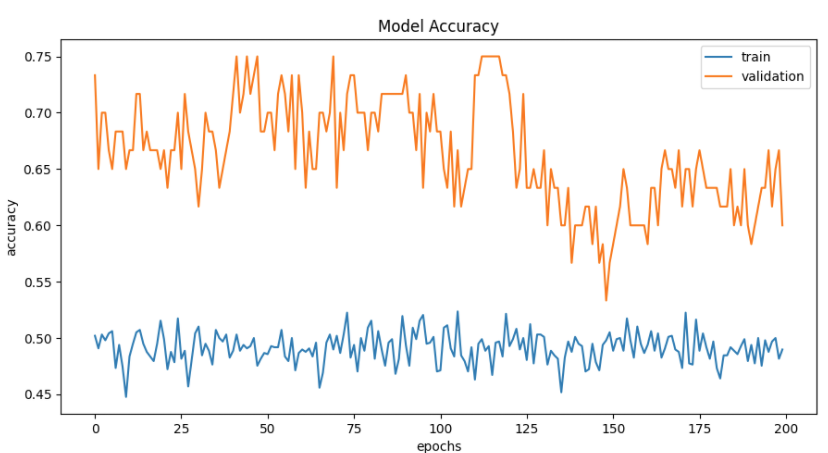
\includegraphics[scale=0.4]{2.png}
\section{Results}
\par
Our initial model with a regular deep learning architecture had an accuracy of ~30\% on the test data. Since it was only trained on ~10\% of the full dataset and the test set came from a different distribution than the training set, this result was expect. Even though random guessing has an accuracy of 50\%, the model was fit to the training data and was unable to generalize at all to the test set.
Our 3D CNN model was trained on the full data for 200 epochs. This model was tuned for accuracy on the validation set, which comes from the same distribution as the test set. It had an accuracy of ~50\% on the training set, ~75\% on the validation set, and 70\% on the test set. 
\par
The evaluations done in the open trials of \textit{'CT-GAN: Malicious tampering of 3D medical imagery using deep learning'} involved 4 detectors (radiologists of 2, 5, 7 years of experience and AI) locating areas of true/false cancers and true/false benign areas. The average false positive (detected fake cancer) rate
was 99.2\% and the average false negative (detected no cancer given real cancer
was removed) 95.8\%.
\par
This task is much more complex than the binary classification task of our research. However, since we have no other alternatives for an optimal classifier proxy, we will compare our results to this accordingly. 
\par
In comparison, our 70\% accuracy for our first 3D CNN model looks promising. It is possible that further tuning and refinement of the same model can make improvements on this number. However, we believe taking an entirely different approach would be better. Our model is tasked with classifying tampered images given that the image has no cancers and has many cancers. The image looks completely different in benign scans versus cancerous scans. Our model may be having trouble in detecting tampering because areas of tampering may look significantly different in healthy and unhealthy scans. This was our observation after working with the data, but an in-depth texture analysis of the images would most likely provide key insights. 
\par
Separating the full tamper detection into three tasks makes more sense intuitively and should be the focus of future research. The first task is cancer detection followed by the second task of tamper detection, therefore the first model is for detecting malignant or benign cancer. One tamper detection model would learn to detect tampering given cancers. Lastly, another model would learn to detect tampering given no cancers. 
\section{Related Work}
Primarily inspired by [1], our work largely models theirs, however our concentration was on improving the accuracy of the model's predictions. Thanks to Minsky et al., we were able to simplify our data preprocessing and accomplish our task with some degree of success in a timely manner.
\par
For our 3D CNN architecture, our team replicated the architecture used in a tuberculosis detection research. Both datasets are very similar as they are 3D CT scans of healthy/unhealthy lungs, which allowed us to also replicate their data transformation process. Additionally, both data was 3-dimensional. Our team believed that the tasks were identical enough so that their architecture might provide us a good starting point for our first model. 
\section{Conclusion}
Some takeaways from this research were the level of commitment required to effectively undertake such a task and produce results, initial experience required for breaking into this area of machine learning, and knowledge of popular machine learning tools such as Keras and Tensorflow. Additionally, we gained familiarity with the GCP environment where in which we utilized an Nvidia Tesla K80 GPU to speed up the process. Each of these aspects are invaluable for contributing to research in the medical field.
\par
As mentioned before, we will continue our research by investigating the three-task solution proposed. It is uncertain at this moment whether it will pay off, but it appears to be the next best objective for us moving forward.

\section{References}
\begin{thebibliography}{9}
    \bibitem{study}
    Mirsky, Yisroel, et al. 'CT-GAN: Malicious tampering of 3D medical imagery using deep learning.' 28th {USENIX} Security Symposium ({USENIX} Security 19). 2019.
    
    \bibitem{original}
    Hasib Zunair, Aimon Rahman, Nabeel Mohammed, Joseph Paul Cohen. 'Uniformizing Techniques to Process CT scans with 3D CNNs for Tuberculosis Prediction' (2020).
    
\end{thebibliography}

\section{Materials}
Our supporting latex files and source-code can be found at https://github.com/viksirivong/MedicalImageTamperDetection.

\end{document}